\documentclass[zihao=false,fontset=windows]{ctexart}
% ctexart 不接受任意 pt 选项。正文改 {10pt}，方括号里是行距。
\usepackage{scrextend}
\changefontsizes[12pt]{10pt}

\usepackage[a4paper,left=2.35cm,right=2.35cm,top=1.7cm,bottom=1.9cm]{geometry}
\usepackage{xcolor}
\usepackage{graphicx}
\usepackage{amsmath,amssymb}
\usepackage{enumitem}
\usepackage{tabularx}
\usepackage{needspace}
\usepackage{colortbl}
\usepackage{listings}
\usepackage{hyperref}
\usepackage[most]{tcolorbox}

\definecolor{feishuText}{RGB}{31,35,41}
\definecolor{feishuBlue}{RGB}{36,91,219}
\definecolor{feishuRed}{RGB}{216,57,49}
\definecolor{feishuGray}{RGB}{100,106,115}
\definecolor{feishuGray2}{RGB}{143,149,158}
\definecolor{feishuPinkBg}{RGB}{251,191,188}
\definecolor{quoteBar}{RGB}{51,112,255}
\definecolor{codebg}{RGB}{245,246,247}
\definecolor{codeborder}{RGB}{222,224,227}
\definecolor{inlinebg}{RGB}{242,243,245}
\definecolor{callRed}{RGB}{253,226,226}
\definecolor{callOrange}{RGB}{255,245,235}
\definecolor{callYellow}{RGB}{254,255,240}
\definecolor{callGreen}{RGB}{240,251,239}
\definecolor{callBlue}{RGB}{240,244,255}
\definecolor{callRedSoft}{RGB}{254,241,241}
\definecolor{callSun}{RGB}{255,255,204}
\definecolor{tableHead}{RGB}{242,243,245}
\definecolor{tableRule}{RGB}{222,224,227}
\definecolor{codeText}{RGB}{31,35,41}
\definecolor{codeKeyword}{RGB}{0,0,255}
\definecolor{codeComment}{RGB}{0,128,0}
\definecolor{codeString}{RGB}{163,21,21}

\setmainfont{Times New Roman}
\setCJKmainfont{Microsoft YaHei}[AutoFakeBold=2.2]
\setCJKsansfont{Microsoft YaHei}[AutoFakeBold=2.2]
\setCJKmonofont{Microsoft YaHei}[AutoFakeBold=2.2]
\setmonofont{Consolas}
\newfontfamily\emojifont{Segoe UI Emoji}

\hypersetup{
  colorlinks=true,
  urlcolor=feishuBlue,
  linkcolor=feishuBlue,
  unicode=true,
  pdftitle={DeepSeek VL2}
}

\setlength{\parindent}{0pt}
\setlength{\parskip}{0.42em}
\setlength{\fboxsep}{1.5pt}
\setlength{\emergencystretch}{3em}
\linespread{1.28}
\color{feishuText}
\arrayrulecolor{tableRule}
\urlstyle{same}

\setlist[enumerate]{label=\textcolor{feishuBlue}{\arabic*.}, leftmargin=1.7em, itemsep=0.22em, topsep=0.28em, parsep=0.08em, partopsep=0pt}
\setlist[itemize,1]{label=\textcolor{feishuBlue}{\textbullet}, leftmargin=1.35em, itemsep=0.18em, topsep=0.25em, parsep=0.06em, partopsep=0pt}
\setlist[itemize,2]{label=\textcolor{feishuBlue}{◦}, leftmargin=1.45em, itemsep=0.12em, topsep=0.15em}
\setlist[itemize,3]{label=\textcolor{feishuBlue}{\rule[0.18em]{0.38em}{0.38em}}, leftmargin=1.55em, itemsep=0.1em, topsep=0.12em}

\newcommand{\feiEmoji}[1]{{\emojifont #1}}
\newcommand{\incode}[1]{\colorbox{inlinebg}{\ttfamily\small #1}}
\newcommand{\bigmath}[1]{%
  \begin{center}\large$\displaystyle #1$\end{center}%
}

\lstset{
  language=Python,
  basicstyle=\ttfamily\footnotesize\color{codeText},
  keywordstyle=\color{codeKeyword},
  commentstyle=\color{codeComment},
  stringstyle=\color{codeString},
  showstringspaces=false,
  breaklines=true,
  columns=fullflexible,
  keepspaces=true,
  tabsize=4,
  upquote=true,
  aboveskip=2pt,
  belowskip=0pt,
  xleftmargin=0pt,
  frame=none
}

\tcbset{
  feishubase/.style 2 args={
    enhanced,
    boxrule=0pt,
    arc=8pt,
    left=10pt,
    right=10pt,
    top=7pt,
    bottom=7pt,
    before skip=6pt,
    after skip=6pt,
    colback=#1,
    colframe=#1,
    before upper={\feiEmoji{#2}\hspace{0.45em}\ignorespaces}
  }
}
\newtcolorbox{feishubox}[2]{feishubase={#1}{#2}, breakable}
\newtcolorbox{feishuboxnb}[2]{feishubase={#1}{#2}}

\newtcolorbox{feishuquote}{
  enhanced,
  breakable,
  boxrule=0pt,
  leftrule=3pt,
  arc=0pt,
  colframe=quoteBar,
  colback=white,
  left=8pt,
  right=2pt,
  top=2pt,
  bottom=2pt,
  before skip=4pt,
  after skip=4pt,
  before upper=\color{feishuGray}
}

\newtcolorbox{feishucode}{
  enhanced,
  breakable,
  colback=codebg,
  colframe=codeborder,
  boxrule=0.6pt,
  arc=6pt,
  left=6pt,
  right=6pt,
  top=5pt,
  bottom=4pt,
  before skip=6pt,
  after skip=6pt
}



% Source: https://scnajei2ds6y.feishu.cn/wiki/FxdNwcNQLiL8rckvMT1cUZH1n1c
% Code blocks omitted by user request. Equations visually transcribed from rendered page.


\begin{document}
{\zihao{1}\bfseries DeepSeek VL2\par}


\begin{feishuquote}

支持动态分辨率和极端图片长宽比（found in InfographicVQA, dense OCR, and detailed visual grounding tasks）\par

\end{feishuquote}

\par\Needspace{8\baselineskip}\vspace{0.95em}\noindent{\zihao{-2}\bfseries \textcolor{feishuBlue}{1.}\hspace{0.45em}模型架构}\par\vspace{0.28em}

\begin{center}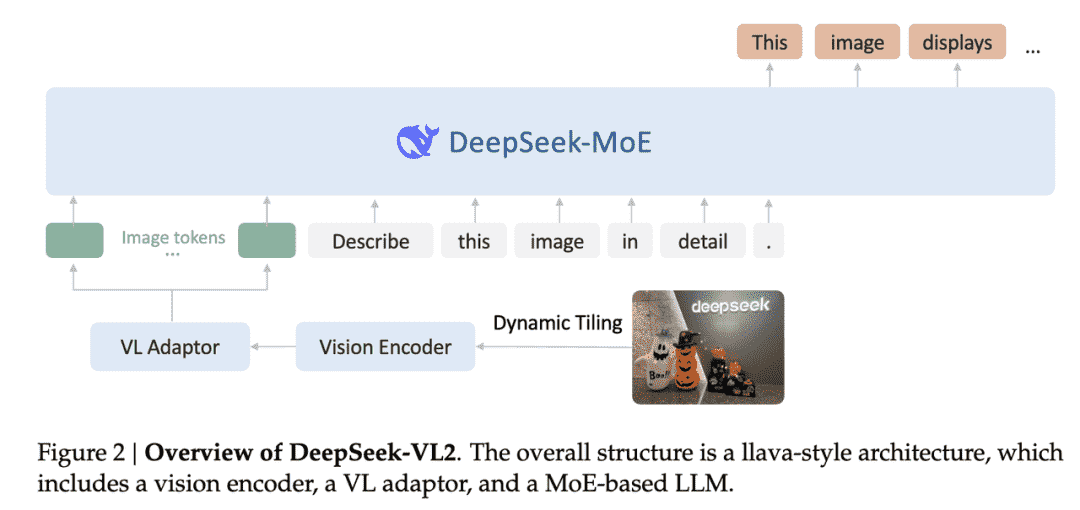
\includegraphics[width=\linewidth,height=0.72\textheight,keepaspectratio]{images/DeepSeek-VL2/fig-01.png}\end{center}

采用的仍然是MLLM主流的Vision Encoder（预训练）+Adaptor桥接+LLM的模型结构。说实话现在MLLM结构基本收敛了（除了InternVL-Xcomposer等会有一些小改动），完全不像从前\href{https://arxiv.org/abs/2204.14198}{Flamingo}那么复杂。\par

值得注意的点是语言模型使用的是DeepSeek V2的MOE模型：\par

\begin{center}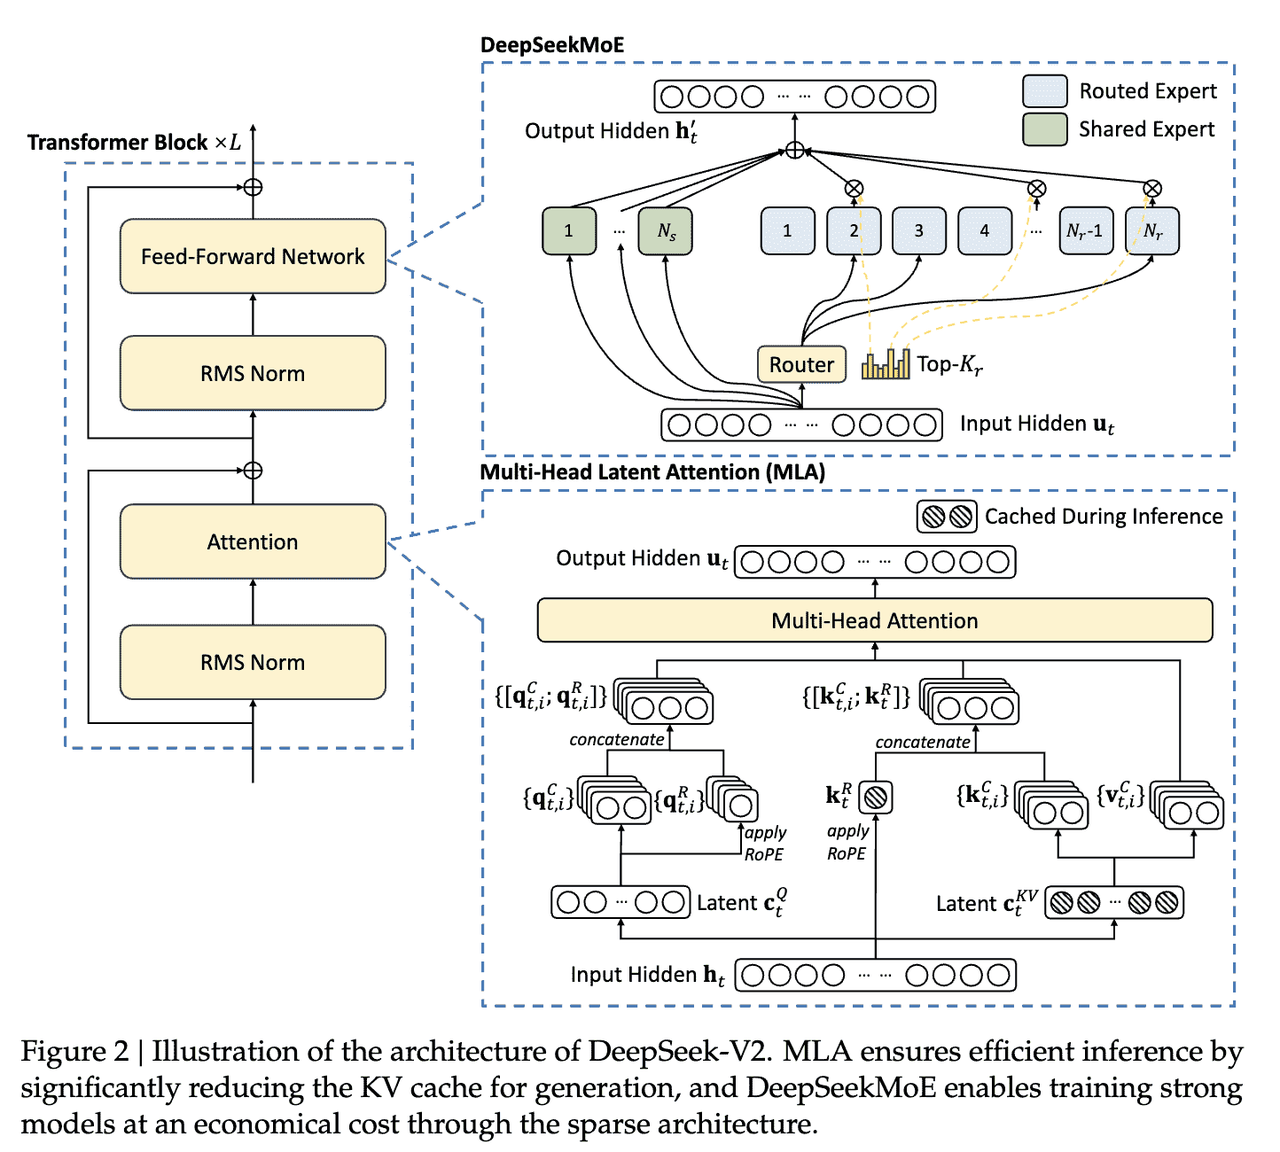
\includegraphics[width=\linewidth,height=0.42\textheight,keepaspectratio]{images/DeepSeek-VL2/fig-02.png}\end{center}

\par\Needspace{8\baselineskip}\vspace{0.95em}\noindent{\zihao{3}\bfseries Vision Encoder}\par\vspace{0.28em}

相比于\href{https://scnajei2ds6y.feishu.cn/wiki/B2SDwuImjimZ4TksKCpcF7e9nnb}{DeepSeek VL}的Hybrid Vision Encoder，DeepSeek-VL2 \textbf{仅使用一个} SigLIP-SO400M 作为图像编码器。\par

\begin{feishuquote}

\begin{itemize}

\item SigLIP-SO400M

\end{itemize}

\textbf{模型架构：} SoViT，结构和ViT一致，但是专注于计算预算一定情况下，对hidden\_dim、width、num\_layers进行scaling。SoViT的形状优化基于以下公式：$x_k^*=\left(\frac{\alpha_k a_k t^c}{\beta_k b_k}\right)^{\frac{1}{b_k+a_k}}$. 其中，$x_k^*$表示最佳形状参数（宽度、深度或MLP维度），$t$为计算预算，$c$为数据扩展指数 。\par

\textbf{训练方式：}SigLIP-SO400M 使用的是前文 (DeepSeek VL-1) 介绍的SigLIP训练方式，其相比与CLIP在loss (CLIP为InfoNCE)上进行了优化：\par

\bigmath{-\frac{1}{|\mathcal B|}\sum_{i=1}^{|\mathcal B|}\sum_{j=1}^{|\mathcal B|}\underbrace{\log\frac{1}{1+e^{z_{ij}(-t\mathbf{x}_i\cdot\mathbf{y}_j+b)}}}_{\mathcal L_{ij}}}

主要优化了两点：1）CLIP由于需要batch的scale，分布式训练时候一次前向需要两次all reduce，sigLIP只需要一次。2）偏置 b 缓解了正负样本不均衡问题。\par

\end{feishuquote}

SigLIP-SO400M 接收分辨率是 384*384，patch\_size 为 14*14，输出shape为 (729, 1152)\par

\par\Needspace{8\baselineskip}\vspace{0.95em}\noindent{\zihao{4}\bfseries Dynamic Tiling Strategy}\par\vspace{0.28em}

其实就是参考了LlavaNext的策略(7)，图像除了resize后进行编码（global thumbnail tile），还会分割成若干384*384的tile（local tile）进行编码，之后直接concat起来。\textbf{所以结合上面SigLIP-SO400M视觉编码器的讲解，每一个tile在编码后产生 27 \(\times\) 27 = 729 个 embedding of 1152 dimensions。}\par

\begin{center}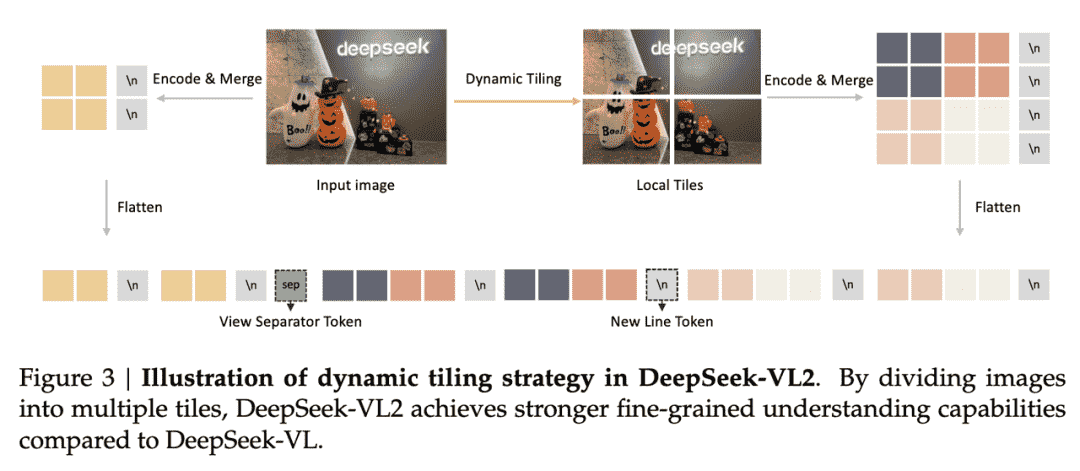
\includegraphics[width=\linewidth,height=0.72\textheight,keepaspectratio]{images/DeepSeek-VL2/fig-03.png}\end{center}

\begin{feishuquote}

注意有一个细节，就是为了控制seqence len，当输入图片数量大于2的时候是禁用Dynamic Tiling Strategy的！\par

\end{feishuquote}

\textbf{注意：这里输出的27\(\times\)27的embedding不是直接展开的！} 会经过 2 \(\times\) 2 的 pixel shuffle operation 压缩到 14 \(\times\) 14 = 196 个 tokens。然后是一些细节性的东西，就是对于两个分割token（<tile\_newline>和<view\_separator>）的插入规则，我给大家总结为三点：\par

\begin{itemize}

\item 对于global thumbnail tile, 每一行自己的embedding遍历完插入一个<tile\_newline>

\item 对于local tile，每一行全局embedding遍历完插入一个<tile\_newline>

\item global thumbnail tile和local tile之间插入一个<view\_separator>

\end{itemize}

设local tile总共有$m_i\times n_i$个，则visual sequence length为 $210+1+m_i\cdot14\times(n_i\cdot14+1)$\par

其中第一个 210 是global tile的 14 \(\times\) 15 = 210\par

\par\Needspace{8\baselineskip}\vspace{0.95em}\noindent{\zihao{3}\bfseries Adaptor}\par\vspace{0.28em}

两层MLP解决。\par

\par\Needspace{8\baselineskip}\vspace{0.95em}\noindent{\zihao{3}\bfseries LLM}\par\vspace{0.28em}

用的是DeepSeek MOE的架构。\par

\begin{center}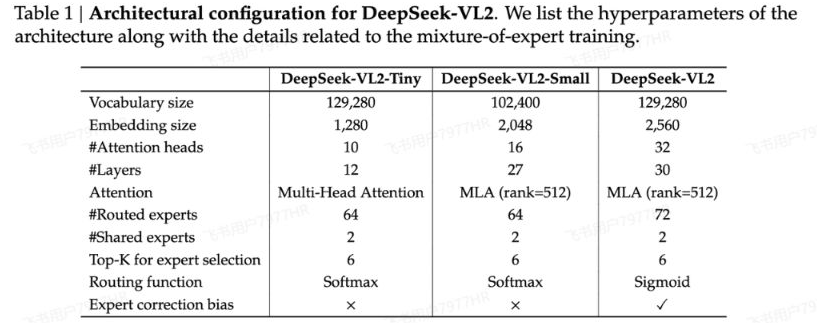
\includegraphics[width=\linewidth,height=0.72\textheight,keepaspectratio]{images/DeepSeek-VL2/fig-04.png}\end{center}

\par\Needspace{8\baselineskip}\vspace{0.95em}\noindent{\zihao{-2}\bfseries \textcolor{feishuBlue}{2.}\hspace{0.45em}实验}\par\vspace{0.28em}

case study可以参考deepseek的blog(8) 。\par

同size模型上表现是能打的。\par

\begin{center}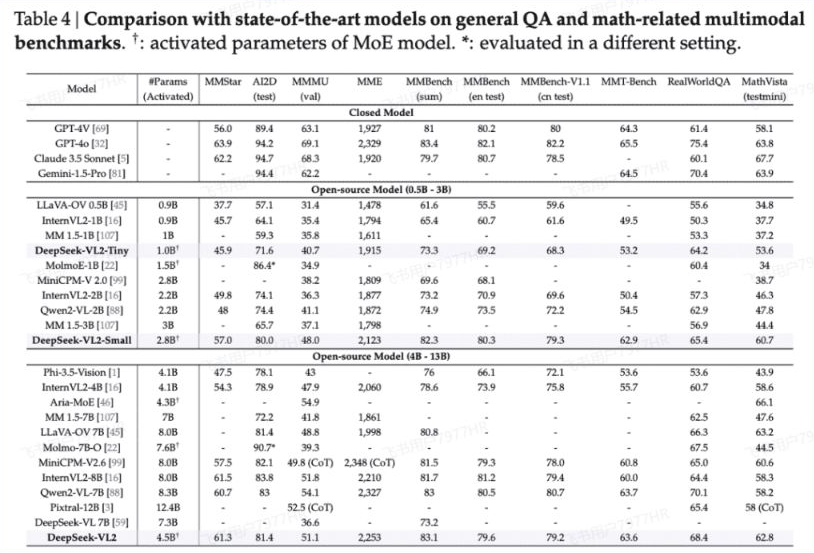
\includegraphics[width=\linewidth,height=0.72\textheight,keepaspectratio]{images/DeepSeek-VL2/fig-05.png}\end{center}

实现同等表现的情况下参数量级大约可以压缩至0.5倍。\par

\begin{center}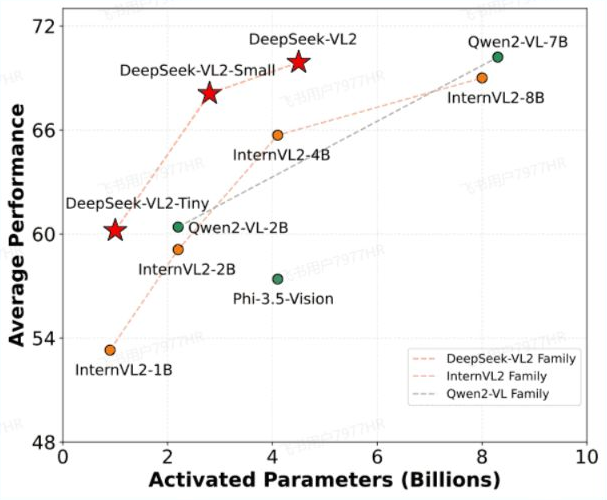
\includegraphics[width=\linewidth,height=0.72\textheight,keepaspectratio]{images/DeepSeek-VL2/fig-06.png}\end{center}

\end{document}